\documentclass[a4paper,12pt]{article}   % papír A4, písmo 12 bodu
\usepackage[utf8x]{inputenc}            %kodovaní UTF-8
\usepackage{ucs}                        %kodovani unicode
\usepackage[czech]{babel}               %podpora cestiny
\usepackage[T1]{fontenc}                %pouzij variantu pisma T1 (hacky, carky)
\usepackage[left=2.5cm,right=1.5cm,top=2.5cm,bottom=2.5cm]{geometry} %okraje stranky
\usepackage{amsmath,amsfonts,amssymb}   %podpora matematiky
\usepackage{gensymb,marvosym}           %symboly celsius (\celsius) apod.
%\usepackage{mathptmx}                   %font Times New Roman s~podporou matematiky
\usepackage{times}                      %font Times New Roman (matematika pismem Computer Modern) 
\usepackage{parskip}                    %mezera mezi odstavci
%\usepackage[document]{ragged2e}         %text zarovany vlevo
\usepackage[none]{hyphenat} \sloppy     %slova nedelit a~nepretekat
\usepackage{titlesec}
\setcounter{secnumdepth}{4}
\clubpenalty 10000                      %kontrolovat sirotky
\widowpenalty 10000                     %kontrolovat vdovy
\usepackage{setspace} \onehalfspacing   %podpora pro zmenu radkovani + radkovani 1,5
\usepackage{enumerate}                  %podpora pro zmenu cislovani
\usepackage{fancyhdr}                   %vlastni zahlavi a~zapati
\usepackage{graphicx}                   %podpora grafiky
\graphicspath{{materialy/}}                   %vychozi adresar s~obrazky
\usepackage{caption}                    %popisky
\usepackage{subcaption}                 %podpopisky
\usepackage{siunitx}
\usepackage{MnSymbol,wasysym}
\usepackage[shortlabels]{enumitem}
\usepackage{amsmath}
\usepackage{lastpage}                   %zjištění poslední stránky \pageref{LastPage}
\usepackage{float}                      
\usepackage{url}
\usepackage[unicode]{hyperref}          %klikaci odkazy v textu
\usepackage{mhchem}
\usepackage{multirow}

\usepackage{halloweenmath}


\titleclass{\subsubsubsection}{straight}[\subsection]
\newcounter{subsubsubsection}[subsubsection]
\renewcommand\thesubsubsubsection{\thesubsubsection.\arabic{subsubsubsection}}
\renewcommand\theparagraph{\thesubsubsubsection.\arabic{paragraph}} % optional useful if paragraphs are to be numbered


%------------------------ čtvrtá a pátá úroveň nadpisu ---------------------------

\titleformat{\subsubsubsection}
  {\normalfont\normalsize\bfseries}{\thesubsubsubsection}{1em}{}
\titlespacing*{\subsubsubsection}
{0pt}{3.25ex plus 1ex minus .2ex}{1.5ex plus .2ex}

\makeatletter

\renewcommand\paragraph{\@startsection{paragraph}{5}{\z@}%
  {3.25ex \@plus1ex \@minus.2ex}%
  {-1em}%
  {\normalfont\normalsize\bfseries}}
\renewcommand\subparagraph{\@startsection{subparagraph}{6}{\parindent}%
  {3.25ex \@plus1ex \@minus .2ex}%
  {-1em}%
  {\normalfont\normalsize\bfseries}}
\def\toclevel@subsubsubsection{4}
\def\toclevel@paragraph{5}
\def\toclevel@paragraph{6}
\def\l@subsubsubsection{\@dottedtocline{4}{7em}{4em}}
\def\l@paragraph{\@dottedtocline{5}{10em}{5em}}
\def\l@subparagraph{\@dottedtocline{6}{14em}{6em}}
\makeatother

\setcounter{secnumdepth}{4}
\setcounter{tocdepth}{4}


\setlist[enumerate]{itemsep=0mm}
%_____________________________|___________________________|_____________________________%
%                             |                           |                             %
%-----------------------------| ZDE VYPLNIT UDAJE O PRACI |-----------------------------%
%_____________________________|___________________________|_____________________________%
%                             

\newcommand{\nazev}{MĚŘENÍ MALÝCH PROUDŮ}                                                        %
\newcommand{\jmeno}{Jakub Dvořák}                                                     %
\newcommand{\datum}{18.10.2020}                                                              %
%---------------------------------------------------------------------------------------%


%-----------------------------| POUŽITÁ MAKRA |-----------------------------%

%\newcommand{\zkratka}{ve výsledku se mi napíše tenhle text}
%\newcommand{}{}
%\newcommand{}{}
%\newcommand{}{}
\newcommand{\tsub}[1]{$_\textrm{#1}$}
\newcommand{\texp}[1]{$^\textrm{#1}$}
\newcommand{\tmu}{$\mu$}
\newcommand{\tpm}{$\pm$}

%_______________________________________________________________________________________%
%_______________________________________________________________________________________%


%----------------------------------- KONEC PREAMBULE -----------------------------------%






%-------------------------------------- DOKUMENT --------------------------------------%
%______________________________________________________________________________________%
\begin{document} %%%%%%%%%%%%%%%%%%%%%%%%%%%%%%%%%%%%%%%%%%%%%%%%%%%%%%%%%%%%%%%%%%%%%%%

\setcounter{page}{0} %cislo strany
\pagestyle{empty} %stranku necislovat

%prostredi pro grafy a schemata \begin{graf} \begin{schema}
\newfloat{schema}{htbp}{schema}\floatname{schema}{Schéma}
\newfloat{graf}{htbp}{graf}\floatname{graf}{Graf}

\begin{titlepage}
    \begin{center}
        \vspace*{1cm}
            
        \Huge
        \textbf{\nazev}
            
        \vspace{0.5cm}
        \LARGE
            
        \vspace{1.5cm}
            
        \textbf{\jmeno}
            
        \vfill
            
        \vspace{0.8cm}
            
        \Large
            
        \datum\\
        \vspace*{.5cm}
        
\includegraphics[width=.4\textwidth]{logo-cvut-fee.png}\\
    \end{center}
\end{titlepage}

% --- definice zapati a~cislovani ---
\newpage 
\pagestyle{fancy}                                       %vlastni zahlavi/zapati
\renewcommand{\headrulewidth}{0pt}                      %bez linky v~zahlavi
\renewcommand{\footrulewidth}{.5pt}                    %linka v~zapati - optional
\lhead{}       \chead{} \rhead{}                        %pole zahlavi (prazdna)
\lfoot{\nazev} \cfoot{} \rfoot{\thepage}   %pole zapati


%------------------------------------ VLASTNÍ TEXT ------------------------------------%



\section{Úkol měření}

\label{zadani}
\begin{enumerate}
    \item V zapojení podle obr. \ref{fig:schema} změřte proud germaniovou diodou v propustném směru v oblasti malých napětí (20 až 100 mV) v pěti bodech charakteristiky:\label{jedna}
    \begin{enumerate}[label=\alph*)]
        \item analogovým mikroampérmetrem,\label{analog}
        \item číslicovým mikroampérmetrem na různých rozsazích,\label{digital}
        \item pomocí převodníku proud - napětí s operačním zesilovačem, u něhož před měřením určete velikost odporu zpětnovazebního rezistoru R tak, aby převod proud - napětí byl 10\texp{-5} A/V.
    \end{enumerate}
    \item Naměřené hodnoty vyneste do společného grafu.
    \item Při měření dle \ref{jedna}\ref{analog} a \ref{jedna}\ref{digital} určete chybu metody způsobenou vnitřním odporem ampérmetru.
    \item Z naměřených hodnot určete \textbf{vnitřní odpory použitých mikroampérmetrů}.
\end{enumerate}



\section{Schéma zapojení}

\label{schema_zapojeni}
\begin{figure}[h!]
    \centering
    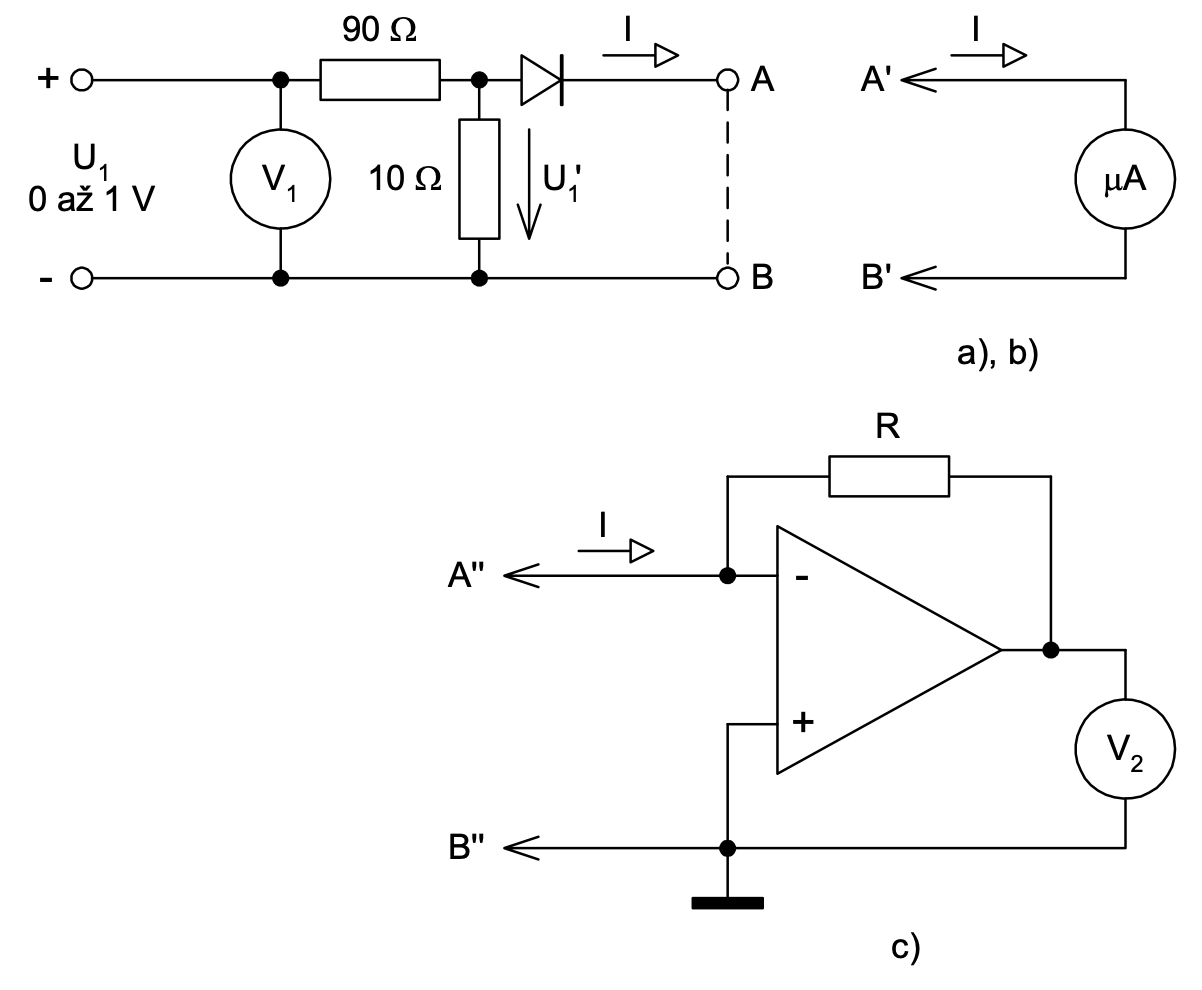
\includegraphics[width=.8\textwidth]{schema.png}
    \caption{Zapojení pro měření malých proudů \cite{navod}}
    \label{fig:schema}
\end{figure}



\section{Seznam použitých přístrojů}

\begin{itemize}
    \item V\tsub{2} - voltmetr číslicový, typ ..., přesnost ...
    \item $\mu$A\tsub{1} - mikroampérmetr magnetoelektrický, tř.přes. 0,5, rozsah 150 \tmu A
    \item $\mu$A\tsub{2} - mikroampérmetr číslicový, typ GDM-8145 přesnost \tpm (0,3 \% z rozsahu + 4 digity), rozsah 200\,\tmu A a 2\,mA
    \item R - přesný rezistor nebo odporová dekáda, přesnost 0,1\,\% (příp. 0,2\,\%)
    \item Př1 - přípravek s odporovým děličem a polovodičovou diodou
    \item Př2 - přípravek s operačním zesilovačem
    \item U\tsub{1} - zdroj proměnného stejnosměrného napětí s číslicově nastavitelnou hodnotou 
    \item NZ - napájecí zdroj pro OZ
\end{itemize}



\section{Teoretický úvod}

Při měření malých proudů ručními ampérmetry nastává chyba měření. Ta je dána relativně vysokým odporem bočníku ampérmetru, na kterém měříme úbytek napětí. Dle obrázku \ref{fig:schema} je vidět, že odpor diody, která není vlivem nízkého napětí zcela otevřena, je srovnatelný s odporem ampérmetru. Vinou čehož vznikne dělič napětí se srovnatelnými úbytky napětí na diodě a na ampérmetru. Tato chyba metody jde kompenzovat zvýšením rozsahu a tedy snížením odporu. Zde se ale naměřená hodnota dostane na začátek rozsahu a vzniká zde opět nejistota měření daná \textit{chybou rozsahu}. 



\section{Naměřené hodnoty}

Změřená data jsou v tabulce \ref{tab:zmereno}.
\begin{table}[h!]
    \centering
    \begin{tabular}{|c|c|c|c|c|}
        \hline
        \rule{0pt}{2.5ex}
        \multirow{2}{*}{Vstupní napětí $\frac{U}{\textrm{V}}$}& Ručičkový \tmu ampérmetr$\frac{I}{\mu\textrm{A}}$ 	&GDM-8145 $\frac{I}{\mu\textrm{A}}$	&GDM-8145 $\frac{I}{\textrm{mA}}$	&IU Převodník $\frac{U}{\textrm{V}}$  \\[.7ex]
        & rozsah  150~μA & rozsah 200~μA & rozsah  2~mA & rozsah  2 V\\\hline\hline
        0,2 &0,9    &1,33   &0,0012 &-0,0155     \\\hline
        0,3 &1,4    &2,36   &0,0024 &-0,0277     \\\hline
        0,4 &2      &3,69   &0,0041 &-0,0448       \\\hline
        0,5 &2,6    &5,39   &0,0064 &-0,0684     \\\hline
        0,6 &3,3    &7,48   &0,0095 &-0,1012     \\\hline
        0,7 &4      &10     &0,0136 &-0,1459         \\\hline
        0,8 &4,8    &12,96  &0,0190 &-0,2062    \\\hline
        0,9 &5,25   &16,37  &0,0260 &-0,2867   \\\hline
        1   &6,4    &20,23  &0,0349 &-0,3926      \\\hline
    
    \end{tabular}
    \caption{Změřené hodnoty}
    \label{tab:zmereno}
\end{table}

Námi změřené hodnoty mají různé předpony i jednotky. Je proto nutné je přepočítat na jednotné jednotky. Pro číslicový ampérmetr stačí hodnoty v mA vynásobit 1000, abychom dostali \tmu A. Pro spočtení napětí na výstupu operačního zesilovače platí:
\begin{equation}
    \begin{split}
        I_{in}&=-I_{out}\\
        I_{in}&=-\frac{U_{out}}{R}\\
        I_{in}&=-\frac{U_{out}}{10\,000} \textrm{A},\\
    \end{split}
    \label{eq:iu}
\end{equation}
kde $I_{out}$ je proud protékající diodou, $U_{out}$ je měřené napětí a $R$ je rezistor připojen mezi výstup a invertující vstup operačního zesilovače.



\section{Zpracování naměřených hodnot}

\subsection{Převod na stejné jednotky}
Jelikož hodnoty napětí byly měřeny ve voltech a jednotné jednotky jsou \tmu A, je potřeba změřené napětí vydělit $-0,1\,\frac{\textrm{A}}{\textrm{V}}$. Přepočtené hodnoty jsou zapsána v tabulce \ref{tab:prepocteno} a zobrazena v grafu \ref{graf:hodnoty}.

\begin{table}[h!]
    \centering
    \begin{tabular}{|c|c|c|c|c|}
        \hline
        \rule{0pt}{2.5ex}
        \multirow{2}{*}{Napětí na děliči $\frac{U}{\textrm{V}}$}& Ručičkový \tmu ampérmetr$\frac{U}{\mu\textrm{A}}$ 	&GDM-8145 $\frac{U}{\mu\textrm{A}}$	&GDM-8145 $\frac{U}{\mu\textrm{A}}$	&IU Převodník $\frac{I}{\mu\textrm{A}}$  \\[.7ex]
        & rozsah  150~μA & rozsah 200~μA & rozsah  2~mA & rozsah  2 V\\\hline\hline
        0,02    &0,9    &1,33   &1,2    &1,55   \\\hline
        0,03    &1,4    &2,36   &2,4    &2,77   \\\hline
        0,04    &2      &3,69   &4,1    &4,48   \\\hline
        0,05    &2,6    &5,39   &6,4    &6,84   \\\hline
        0,06    &3,3    &7,48   &9,5    &10,12  \\\hline
        0,07    &4      &10     &13,6   &14,59  \\\hline
        0,08    &4,8    &12,96  &19     &20,62  \\\hline
        0,09    &5,25   &16,37  &26     &28,67  \\\hline
        0,1     &6,4    &20,23  &34,9   &39,26  \\\hline
    \end{tabular}
    \caption{Přepočtené hodnoty}
    \label{tab:prepocteno}
\end{table}

Nejistotu pro ručičkový ampérmetr spočítáme pomocí vzorce
\begin{equation}
    u(I_{rv}) = \frac{TP\cdot rozsah}{100\cdot\sqrt{3}} = \frac{0,5\cdot 150\cdot 10^{-6}}{100\cdot\sqrt{3}} = 0,433 \mu ~\textrm{A.}
\end{equation}

Nejistotu pro číslicový ampérmetr s rozsahem 200\,μA spočítáme následovně:
\begin{equation}
    i(I_{čv}) = \frac{\delta_1 X + \delta_2 M}{100\sqrt{3}} = \frac{0,3\%\cdot I+2\cdot\frac{200}{20000}}{100\sqrt{3}}\,\mu \textrm{A}
\end{equation}
a pro rozsah 2\,mA
\begin{equation}
    i(I_{čv}) = \frac{\delta_1 X + \delta_2 M}{100\sqrt{3}} = \frac{0,3\,\%\cdot I[\mu \textrm{A}]+2\cdot\frac{2\cdot 10^3}{20000}}{100\sqrt{3}}\, \mu \textrm{A.}
\end{equation}

Výsledné nejistoty jsou v tabulce \ref{tab:nejistoty}.
\begin{table}
    \centering
    \begin{tabular}{|c|c|c|}
        \hline
        \multirow{2}{*}{Napětí na děliči}& GDM-8145 	&GDM-8145 \\[.7ex]
        & rozsah 200~μA & rozsah  2~mA \\\hline\hline
        0,02&0,000139&0,001175\\\hline
        0,03&0,000156&0,001196\\\hline
        0,04&0,000179&0,001226\\\hline
        0,05&0,000209&0,001266\\\hline
        0,06&0,000245&0,001319\\\hline
        0,07&0,000289&0,001390\\\hline
        0,08&0,000340&0,001484\\\hline
        0,09&0,000399&0,001605\\\hline
        0,10&0,000466&0,001759\\\hline
    \end{tabular}
    \caption{Nejistoty měření pro různé rozsahy a hodnoty}
    \label{tab:nejistoty}
\end{table}

\begin{graf}[h!]
    \centering
    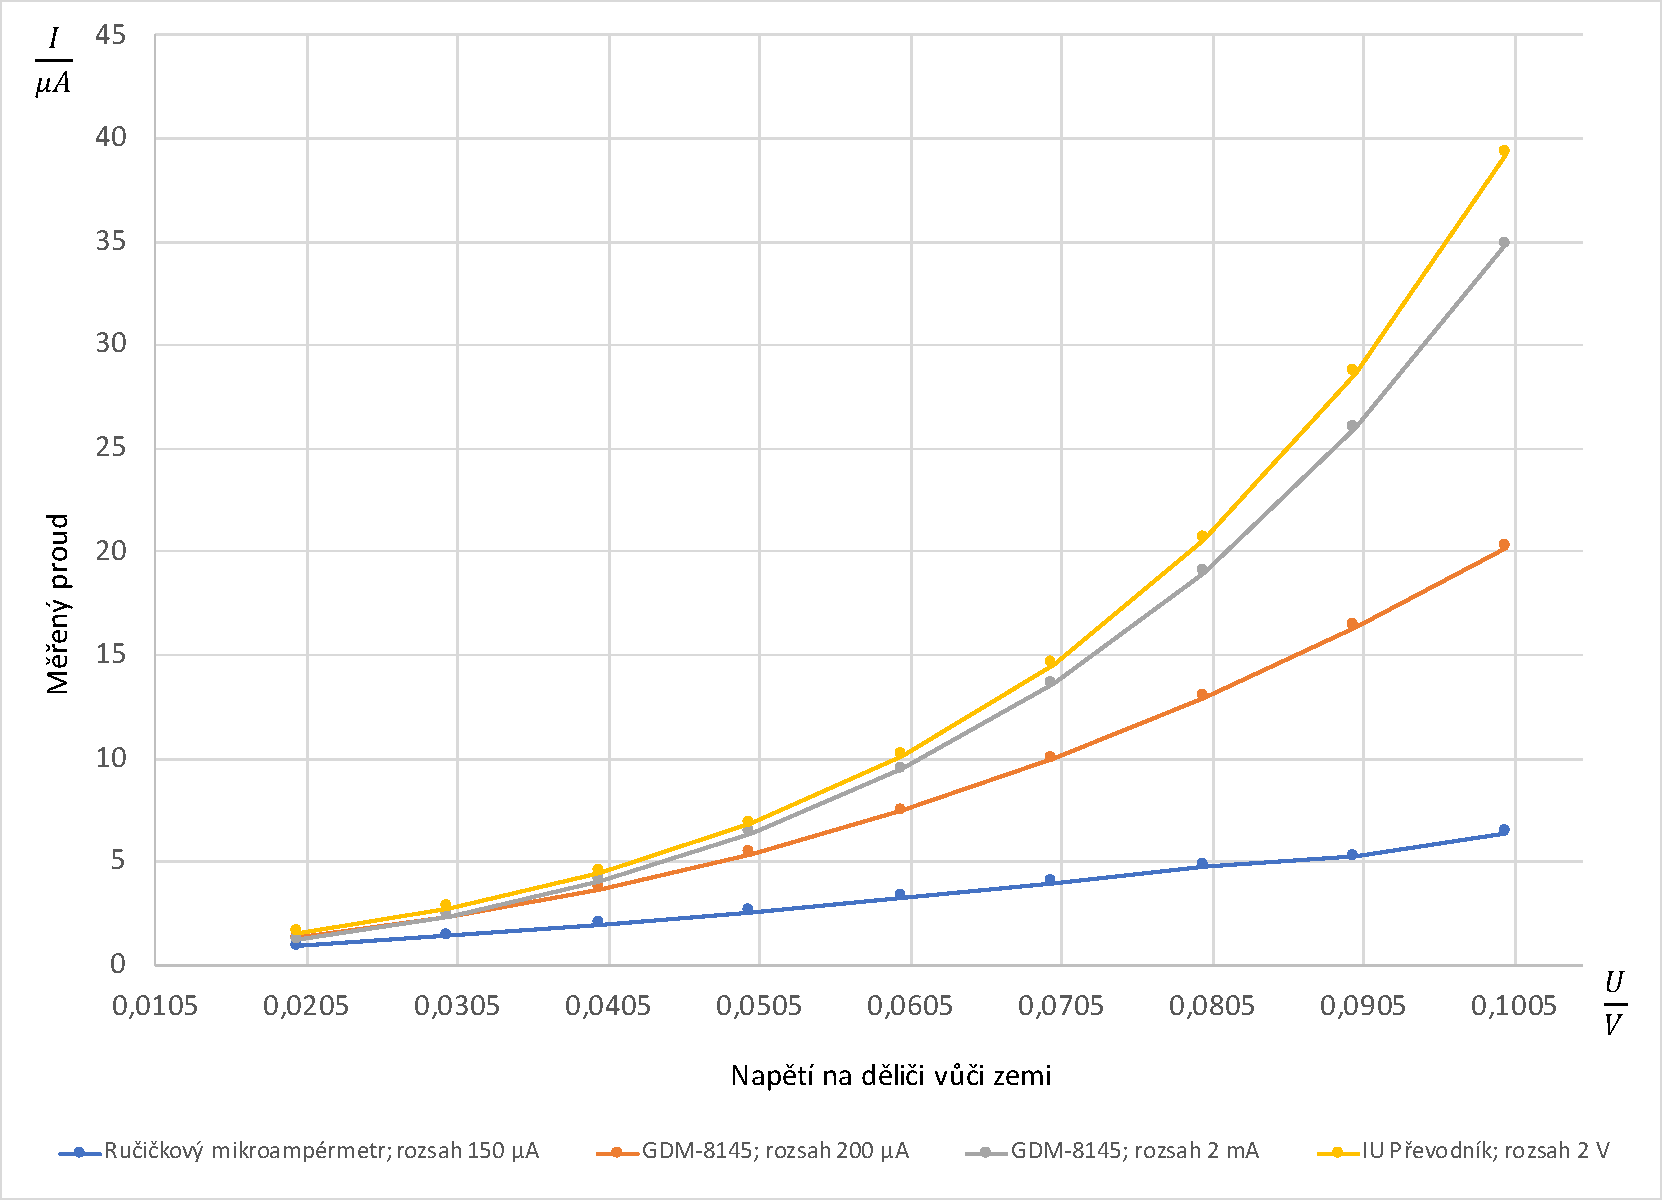
\includegraphics[width=.8\textwidth]{graf_namereno.pdf}
    \caption{Naměřené hodnoty přepočtené na \tmu A}
    \label{graf:hodnoty}
\end{graf}

\subsection{Nejistota IU převodníku}
Pro určení nejistoty měření proudu z měření napětí musíme parciálně zderivovat rovnici \ref{eq:iu} podle všech proměnných. Celý postup je v rovnici \ref{eq:oz_nejistota}.
\begin{equation}
    \begin{split}
        u_{OZ}(I_{oz})&=\sqrt{\left(\frac{\partial I}{\partial R} \cdot u(R)\right)^2+\left(\frac{\partial I}{\partial U} \cdot u(U)\right)^2+\left(u(I_0)\right)^2}\\
        u_{OZ}(I_{oz})&=\sqrt{\left(-\frac{U}{R^2}\cdot u(R)\right)^2+\left(\frac{1}{R}\cdot u(U)\right)^2+\left(u(I_0)\right)^2}\\
    \end{split}
    \label{eq:oz_nejistota}
\end{equation}
Po dosazení dostaneme:
\begin{equation*}
    u_{OZ}(I_{oz})=\sqrt{\left(\frac{U}{R^2}\cdot u(R)\right)^2+\left(-\frac{1}{R}\cdot u(U)\right)^2+\left(u(I_0)\right)^2}
\end{equation*}

\subsection{Chyba měření mikroampérmetrů}
Pro zjištění relativní hodnoty musíme nejdříve znát absolutní chybu $\Delta_{\textrm{met}}$, kterou spočítáme jako
\begin{equation}
    \Delta_{\textrm{met}} = N - S.
    \label{eq:abs}
\end{equation}
Absolutní chybu metody následně spočítáme pomocí rovnice 
\begin{equation}
    \delta_{\textrm{met}} = \frac{\Delta_{\textrm{met}}}{S}.
    \label{eq:rel}
\end{equation}
Rovnice \ref{eq:rel} jde poté upravit do tvaru:
\begin{equation}
    \delta_{\textrm{met}} = \frac{N-S}{S},
\end{equation}
kde $N$ je naměřená hodnota a $S$ je skutečná hodnota. Jelikož jsme stanovili odpor UI převodníku za nulový, můžeme hodnotu jím naměřenou považovat za skutečnou a hodnotu naměřenou ručičkovým resp. číslicovým ampérmetrem s ní porovnávat.

Jednotlivé relativní chyby pro analogový ampérmetr a číslicový ampérmetr s dvěma různými rozsahy jsou v tabulce \ref{tab:rel}.

\begin{table}[h!]
    \centering
    \begin{tabular}{|c|c|c|c|}
        \hline
        \rule{0pt}{2.5ex}
        \multirow{2}{*}{Napětí na děliči} &Ručičkový \tmu ampérmetr	&GDM-8145 	&GDM-8145 \\[.7ex]
        & rozsah  150~μA & rozsah 200~μA & rozsah  2~mA \\\hline\hline
        0,02 & -0,4194 & -0,1419 & -0,2258 \\\hline
        0,03 & -0,4946 & -0,1480 & -0,1336 \\\hline 
        0,04 & -0,5536 & -0,1763 & -0,0848 \\\hline 
        0,05 & -0,6199 & -0,2120 & -0,0643 \\\hline
        0,06 & -0,6739 & -0,2609 & -0,0613 \\\hline
        0,07 & -0,7258 & -0,3146 & -0,0679 \\\hline
        0,08 & -0,7672 & -0,3715 & -0,0786 \\\hline
        0,09 & -0,8169 & -0,4290 & -0,0931 \\\hline
        0,1  & -0,8370 & -0,4847 & -0,1111 \\\hline
    \end{tabular}
    \caption{Relativní chyby metody}
    \label{tab:rel}
\end{table}
V absolutní hodnotě jsou data v tabulce \ref{tab:rel_percent}
\begin{table}[h!]
    \centering
    \begin{tabular}{|c|c|c|c|}
        \hline
        \rule{0pt}{2.5ex}
        \multirow{2}{*}{Napětí na děliči} &Ručičkový \tmu ampérmetr	&GDM-8145 	&GDM-8145 \\[.7ex]
        & rozsah  150~μA & rozsah 200~μA & rozsah  2~mA \\\hline\hline
        0,02&41,94&14,19&22,58  \\\hline
        0,03&49,46&14,80&13,36  \\\hline
        0,04&55,36&17,63&8,48   \\\hline
        0,05&61,99&21,20&6,43   \\\hline
        0,06&67,39&26,09&6,13   \\\hline
        0,07&72,58&31,46&6,79   \\\hline
        0,08&76,72&37,15&7,86   \\\hline
        0,09&81,69&42,90&9,31   \\\hline
        0,10&83,70&48,47&11,11  \\\hline
    \end{tabular}
    \caption{Relativní chyby metody v procentech}
    \label{tab:rel_percent}
\end{table}
Chyba metody je zobrazena v grafu \ref{graf:chyba}.
\begin{graf}
    \centering
    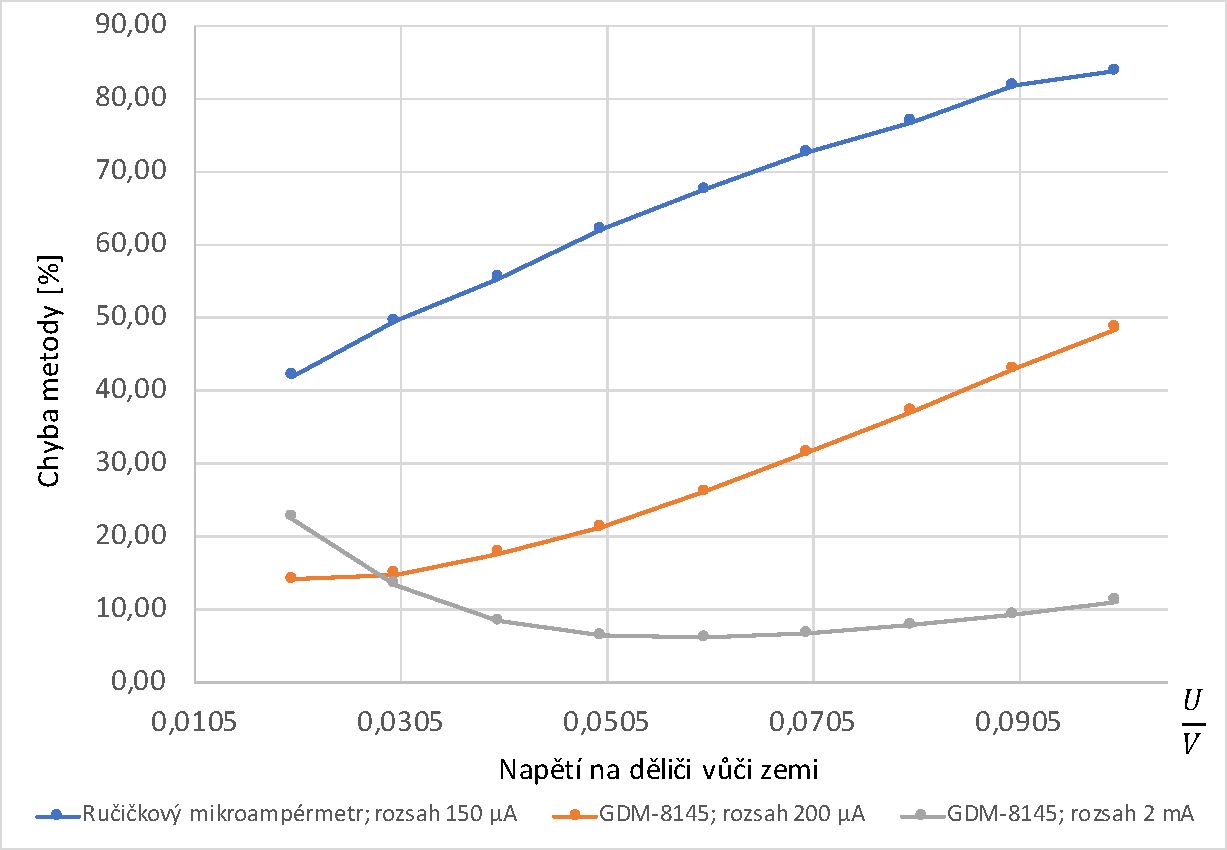
\includegraphics[width=.8\textwidth]{graf_chyba.pdf}
    \caption{Relativní chyba metody v závislosti na měřeném napětí}
    \label{graf:chyba}
\end{graf}
Z tabulky \ref{tab:rel} můžeme spočítat nejistotu podle vzorce \ref{eq:chyba2nejistota}, čímž dostaneme tabulku \ref{tab:chyba2nejistota}.
\begin{equation}
    u_b(I)=\frac{\Delta}{\sqrt{3}}
    \label{eq:chyba2nejistota}
\end{equation}
\begin{table}[h!]
    \centering
    \begin{tabular}{|c|c|c|c|}
        \hline
        \rule{0pt}{2.5ex}
        \multirow{2}{*}{Napětí na děliči} &Ručičkový \tmu ampérmetr	$\frac{U}{\mu\textrm{A}}$&GDM-8145 	$\frac{U}{\mu\textrm{A}}$&GDM-8145 $\frac{U}{\mu\textrm{A}}$\\[.7ex]
        & rozsah  150~μA & rozsah 200~μA & rozsah  2~mA \\\hline\hline
        0,02 & 0,2421 & 0,0819 & 0,1304 & \\\hline
        0,03 & 0,2855 & 0,0855 & 0,0771 & \\\hline
        0,04 & 0,3196 & 0,1018 & 0,0490 & \\\hline
        0,05 & 0,3579 & 0,1224 & 0,0371 & \\\hline
        0,06 & 0,3891 & 0,1506 & 0,0354 & \\\hline
        0,07 & 0,4191 & 0,1816 & 0,0392 & \\\hline
        0,08 & 0,4430 & 0,2145 & 0,0454 & \\\hline
        0,09 & 0,4716 & 0,2477 & 0,0538 & \\\hline
        0,10 & 0,4832 & 0,2799 & 0,0641 & \\\hline
    \end{tabular}
    \caption{Nejistota měření vypočtená z chyby měření}
    \label{tab:chyba2nejistota}
\end{table}

\subsection{Měření vnitřního odporu ampérmetru}
Pro jednotlivé kroky napětí použijeme ohmův zákon pro výpočet odporu diody a tento odpor následně odečteme od celkového odporu tj. i s ampérmetrem. Platí tedy následující rovnice:
\begin{equation}
    R_A=\frac{U}{I_A} - \frac{U}{I_ref},
\end{equation}
kde $U$ je napětí na děliči, $I_A$ je proud změřený ampérmetrem, který nás zajímá a $I_{ref}$ je referenční hodnota proudu - proud změřená UI převodníkem. Dosazením dat do vzorce dostaneme následující tabulku \ref{tab:odpor} a graf \ref{graf:odpor}.
\begin{table}[h!]
    \centering
    \begin{tabular}{|c|c|c|c|}
        \hline
        \rule{0pt}{2.5ex}
        \multirow{2}{*}{Napětí na děliči} &Ručičkový \tmu ampérmetr	$\frac{R}{\Omega}$ &GDM-8145 $\frac{R}{\Omega}$	&GDM-8145 $\frac{R}{\Omega}$\\[.7ex]
        & rozsah  150~μA & rozsah 200~μA & rozsah  2~mA \\\hline\hline
        0,02&9319&2134&3763\\\hline
        0,03&10598&1882&1670\\\hline
        0,04&11071&1912&828\\\hline
        0,05&11921&1966&503\\\hline
        0,06&12253&2093&387\\\hline
        0,07&12702&2202&349\\\hline
        0,08&12787&2293&331\\\hline
        0,09&14004&2359&322\\\hline
        0,10&13078&2396&318\\\hline
    \end{tabular}
    \caption{Spočítaný vnitřní odpor ampérmetrů}
    \label{tab:odpor}
\end{table}

\begin{graf}[h!]
    \centering
    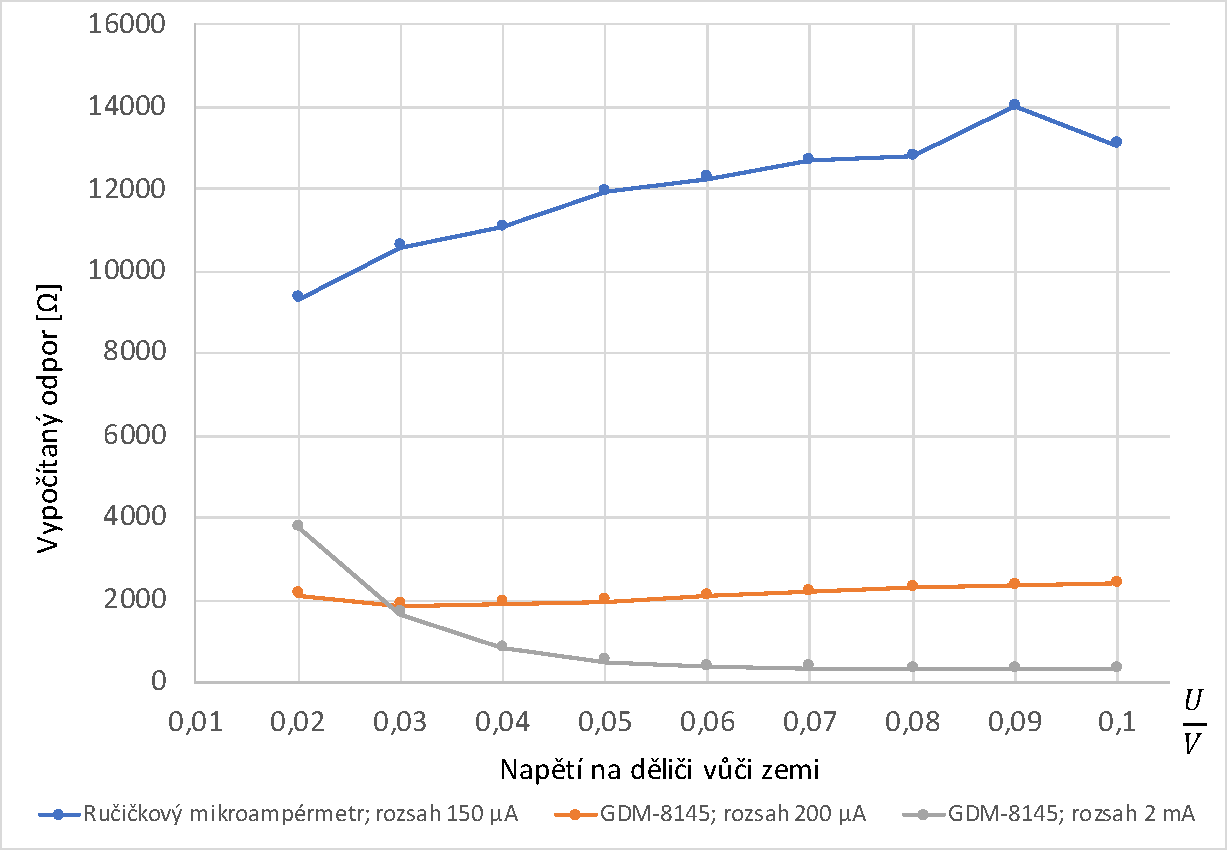
\includegraphics[width=.8\textwidth]{graf_odpor.pdf}
    \caption{Závislost naměřeného odporu na vstupním napětí}
    \label{graf:odpor}
\end{graf}

\section{Závěrečné vyhodnocení}
Zjistili jsme, že při měření malých proudů je měření zatíženo relativně velkou chybou. U ručičkového přístroje relativní chyba dosahovala hodnoty až 83\,\% a u číslicového přístroje šlo o relativní chybu 48\,\% v rozsahu \tmu A a 11\,\% v rozsahu 2\,mA.



%--- LITERATURA a~ZDROJE (povinne) ---
\clearpage
\renewcommand{\refname}{Seznam použité literatury a~zdrojů informací} 
%\section*{Seznam použité literatury a~zdrojů informací}
\phantomsection %pridej odkaz do PDF zalozek
\addcontentsline{toc}{section}{Seznam použité literatury a~zdrojů informací}

\begin{thebibliography}{99}

%----------------------------------------------------
\subsection*{Seznam použitých internetových zdrojů}
    \bibitem{navod} Návod k laboratorní úloze
    
\end{thebibliography}

\end{document}